% Sample Dissertation, Thesis, or Document %
%            for use with the              %
%  University of Arizona Thesis Class,     %
%               uathesis.cls               %
%------------------------------------------%

% We'll use the uathesis document class (duh).  The uncommented line
% below will produce a Dissertation, the others would produce a Thesis
% or a Document.  There are other options available to you like turning
% on the copyright statement and replacing the year on the title page
% with a "generated on" stamp (handy for early drafts).  To find out
% what the available options are, take a look into the uathesis.cls
% file and look for the \DeclareOption commands near the top of that
% file.
% There are five copyright options.  Copyright, no copyright, and three
% different Creative Commons licences.  Use the one you want (If you go
% Creative Commons, I (DM) think the CC-BY-ND makes the most sense)  See
% uathesis.cls for the reason why the non-commercial licenses are not
% included.
\documentclass[dissertation]{uathesis}
%\documentclass[dissertation,copyrig?ht]{uathesis}
%\documentclass[dissertation,CC-BY]{uathesis}
%\documentclass[dissertation,CC-BY-SA]{uathesis}
%\documentclass[dissertation,CC-BY-ND]{uathesis}
%\documentclass[thesis]{uathesis}
%\documentclass[document]{uathesis}

% Package Usage
% These are the packages that we need
\usepackage{pdfpages}
\usepackage{amsmath}
\usepackage{physics}
\usepackage{float}
\usepackage{graphicx}
\usepackage{natbib}			% natbib is available on most systems, and is
					% terribly handy.
					% If you want to use a different Bibliography package, 
					% you should be able to, just change this
					% and the \bibliographystyle command below.  Be warned
					% that you may need to do a little hacking to get
					% the REFERENCES item to show up in your TOC.

% Compatibility with the AASTEX package 
% of the American Astronomical Society.
%\usepackage{deluxetable}		% Allows use of AASTEX deluxe tables
%\usepackage{aastex_hack}		% Allows other AASTEX functionality.

% These are other packages that you might find useful.
% For controlling the fonts, see
% http://www.math.uiuc.edu/~hartke/computer/latex/survey/survey.html
% The following is a nice font set:
%\usepackage{mathtime}			% Times for letters; Belleek math.
%
%\usepackage{amsmath}			% AMS Math (advanced math typesetting)
%\usepackage{lscape}			% Used for making fitting large tables in by putting them landscape
%\usepackage{refs}			
%
% If you are using hyper-ref (recommended), this command must go after all 
% other package inclusions (from the hyperref package documentation).
% The purpose of hyperref is to make the PDF created extensively
% cross-referenced.
\usepackage[bookmarks,colorlinks=true,urlcolor=black,linkcolor=black,citecolor=black]{hyperref}

% Set up some values.
\completetitle{Advances In Physical Systems Modeling Using 
Explicitly Correlated Gaussian Functions}
\fullname{Nikita Kirnosov}			% Grad college wants your full name here.
\degreename{Doctor of Philosophy}	% Title of your degree.

\begin{document}


% Set up the title page
\maketitlepage
{DEPARTMENT OF PHYSICS}	% Title of your department.
{2015}							

% Insert the approval form.  Note that for electronic submission
% of your Ph. D. dissertation, you must bring *two* copies of the
% approval page to your final defense.  These must be signed by
% the committee.  Make two photocopies: one for Pam and the other
% for your records.  Then, bring the two signed originals to the
% graduate college when you submit the final version of the
% dissertation to the University of Arizona.
\approval
{2 Decemder 2015}		% Defense Date	
{Dr. Ludwik Adamowicz}	% Dissertation Director
{Dr. Ludwik Adamowicz}	% 1st committee member
{Dr. Brian Anderson}		% 2nd committee member
{Dr. Andrei Lebed}		% 3rd committee member
{Dr. Srinivas Manne}		% 4th committee member
{Dr. Oliver Monti}		% 5th committee member

% Include the ``Statement by Author'' for Dissertations
\statementbyauthor
% If this is a Thesis, use the following form, with your thesis director's
% name and title in the square brackets like so (you should also omit the 
% approval form insertion above):
%\statementbyauthor[Jane M. Doe\\Professor of Chemistry]

% Include the ``Acknowledgements''
\incacknowledgements{acknowledgements}

% Include the ``Dedication''
%\incdedication{dedication}

% Create a ``Table of Contents''
\tableofcontents

% Create a ``List of Figures''
\listoffigures

% Create a ``List of Tables''
\listoftables

% Include the ``Abstract''
\incabstract{abstract}

% Include the various chapters
\chapter{INTRODUCTION\label{chap1}}

\section{Dissertation Structure}

This dissertation has an article-based format. All the manuscripts produced
during the candidacy are included as appendices. While each manuscript is 
self-contained and self-explanatory, in the context of this dissertation
they would be addressed as sources of the detailed description and more
specific analysis. The goal of this dissertation is to provide a reader 
with good understanding of the method applicability and its' advantages
and disadvantages in comparison to the other methods used for certain
classes of problems. 

In this chapter we will consider general approach to the accurate modeling
of the system wave function with a linear combination of explicitly 
correlated Gaussian functions (ECG). In order to relief the following 
chapters from the technical details, most of the mathematical concepts
are be introduced here. The simplest form of the ECG function is considered
and its properties are discussed. 

In chapter \ref{nonBO} some applications of this method to 
various systems with Coulomb interactions (atoms, molecules, $etc.$)
considered with no Born-Oppenheimer approximation made.
Modifications needed to be made to the basis function for each class
of systems are discussed.

Chapter \ref{prog} contains the description of the code used for calculations
and discusses the nuances of the particular system implementation.
Moreover, some ways of increasing code performance and decreasing space 
requirements are considered.

Finally, chapter \ref{future} gives an overview of  the avenues of research 
opened as a result of the work constituting this dissertation.

\section{Coordinate Frame and Hamiltonian}

A system of $n+1$ particles with masses $M_i$ and charges $Q_i$ can be
described at any moment of time with $n+1$ coordinate vectors  

\begin{align}
    R_i &= 
    \begin{pmatrix}
           x_i \\           
           y_i \\
           z_i
    \end{pmatrix}
\end{align}

and $n+1$ momenta vectors

\begin{align}
    P_i &= 
    \begin{pmatrix}
           p_{x,i} \\           
           p_{y,i} \\
           p_{z,i}
    \end{pmatrix}.
\end{align}

The Hamiltonian operator for this system can be written as 

\begin{equation}
H = \sum_i^{n+1} \frac{P_i^2}{2M_i} + \sum_{i,j>i}^{n+1} \frac{Q_i Q_j}{R_{ij}},
\end{equation}

where

\begin{equation}
R_{ij} = \| R_i - R_j \|.
\end{equation}

It is easy to see that this laboratory frame Hamiltonian includes the center
of mass motion. In order to rigorously separate it out, a transformation 
of the coordinate system should be performed. Instead of considering a system
as $n+1$ particles with charges $Q_{i+1}$ and masses $M_{i+1}$, we will consider 
$n$ pseudo-particles with charges $q_i = Q_{i+1}$ and reduced masses 
$\mu_i = \frac{M_1 M_{i+1}}{M_1 + M_{i+1}}$ moving in the
central field of the reference particle charge $q_0$. 

Figure \ref{coord} illustrates the transition to the internal coordinate frame which 
has its center places on one of the particles. Normally for the reference particle
the most distinguishable (a nucleus in the atom) or the heaviest (deuteron
in HD$^+$) particle is chosen. The position of that particle with respect to the 
laboratory Cartesian coordinate frame is described by a vector $r_0 = R_1$,
and other particles' coordinates are defined with respect to the reference particle:
$r_i = R_1 - R_{i+1}$.

\begin{figure}[H]
\begin{center}
\includegraphics[width=150mm]{../pics/coordinates.png}
\caption[Coordinate frame transformation]{Coordinate frame transformation. \label{coord}}
\end{center}
\end{figure}

The internal Hamiltonian of the considered system now becomes

\begin{equation}
H_{int} = \sum_{i=1}^n \frac{P^{2}_i}{2\mu_i} + \sum_{ i \neq j }^n \frac{P_i P_j}{2 m_0}
+ \sum_{i}^{n} \frac{q_i q_0}{\| r_i \|} + \sum_{i,j>i}^{n} \frac{q_i q_j}{\| r_i - r_j \|}.
\end{equation}

Substituting 

\begin{align}
P_i &= \frac{\nabla_{r_i}}{i} \\
r_{ij} &= r_i - r_j,
\end{align}

we obtain the final form of the internal Hamiltonian operator:

\begin{equation}
H_{int} = -\frac{1}{2} \left( \sum_{i=1}^n \frac{\nabla^2_{r_i}}{\mu_i} + \sum_{ i \neq j }^n \frac{\nabla_{r_i} \nabla_{r_j}}{m_0} \right)
+ \sum_{i}^{n} \frac{q_i q_0}{\| r_i \|} + \sum_{i,j>i}^{n} \frac{q_i q_j}{\| r_{ij} \|}.
\label{intH}
\end{equation}

It can be seen that the fist term of the internal Hamiltonian describes 
individual kinetic energies of the particles, while the third and the fourth
terms are used to take into account the Coulomb interactions between all
charges in the system. Second term is called a mass-polarization term and
originates from the choice of the internal coordinate system, which is
a non-inertial coordinate frame.

This Hamiltonian posses a number of important properties. It 
\begin{enumerate}
  \item describes all particles as quantum particles,
  \item accounts for all interactions,
  \item provides one-step variational approach,
  \item reduces problem dimensionality,
  \item is isotropic.
\end{enumerate}

It has to be mentioned that this Hamiltonian does not include the description 
of relativistic effects and thus should be more accurately called non-relativistic
internal Hamiltonian. The direct inclusion of additional terms to describe
relativistic as well as other interactions is possible in principle.


\section{Explicitly Correlated Gaussian Functions}

Since the Schrodinger equation 
\begin{equation}
H \Psi = E \Psi
\end{equation}
is insoluble by current standards, we have to find a way
around this problem.

One possibility is to expand a wave function in a complete 
set of functions that obey the same boundary conditions:
\begin{equation}
\Psi (r) = \sum_k^{\infty} c_k \phi_k(r),
\end{equation}
where $c_k$ are the linear expansion coefficients.

Note that in the equation above infinity symbol is used to 
communicate the completeness; the actual number of basis functions
does not have to be infinite. Nevertheless, the complete basis
set is not achievable for many cases and has to be truncated:

\begin{equation}
\Phi (r) = \sum_k^{K} c_k \phi_k(r).
\label{wf}
\end{equation}

The wave function representation (\ref{wf}) can be adequate for
an accurate description of a relatively simple and confined 
wave functions with a number of basis functions $K$ being
relatively small. The degree of completeness of such basis set 
may be evaluated by variational principle, which states that 
the expectation value of the Hamiltonian computed with the 
trial function is higher or equal to the true energy value:
\begin{equation}
E = \frac{\expval{H}{\Psi}}{\bra{\Psi}\ket{\Psi}} \leq 
\frac{\expval{H}{\Phi}}{\bra{\Phi}\ket{\Phi}}
\label{var_principle}
\end{equation}

In our work we have chosen to use functions of the following type
as basis functions:
\begin{equation}
\phi_k = \exp \left[ - r' (A_k \otimes I_3) r \right],
\label{simple_gaussian}
\end{equation}
where $r'$ is a row vector of length $3n$ containing pseudo-particles'
coordinates in an internal coordinate frame ($r'=[x_1,y_1,z_1,...,x_n,y_n,z_n]$)
and $A_k$ is $n\times n$ symmetric matrix. Since the function (\ref{simple_gaussian})
must be square-integrable in order to be used for description of the bound states,
the matrix $A_k$ has to be positive definite. That can be achieved through the use
of Cholesky factorization $A_k=L_k L_k'$, where $L_k$ is a lower triangular matrix.
in simplest case, all off-diagonal elements of $A_k$ matrix can be set to zero;
however, in order to describe the correlation effects between the particles,
they should also be optimized. The resulting function would contain the correlation
explicitly and thus be called Explicitly Correlated Gaussian function.

It has to be noticed that according to the Pauli principle, the total wave function
which includes the spin degrees of freedom of a quantum system must either be symmetric 
or antisymmetric with respect to permutations of identical particles. 
Thus, our basis set expansion should take this requirement into account. 
In variational calculations this puts a constraint on the symmetry of the basis 
functions that can be used. 

In general, in order to build properly (anti)symmetric wave functions, we have to deal 
with both the spatial and spin coordinates. Due to the fact that the Hamiltonian of a
nonrelativistic Coulomb system does not depend on the spin of particles, it is possible 
to completely eliminate the spin variables from consideration. The projection operators
$Y$ for irreducible representations of the symmetric group (called Young operators) are 
obtained from their corresponding Young tableaux. Thus, our properly symmetrized 
trial wafe function would have the following form:
\begin{equation}
\Phi (r) = \sum_k^{K} c_k Y \phi_k(r).
\label{wf_perm}
\end{equation}



\section{General Method Description}

All the calculations were performed within the framework of the Ritz variational method. 
The main idea of the variational method in nonrelativistic quantum mechanics is based on 
the fact that the expectation value of the Hamiltonian of the system computed with a
trial wave function is always an upper bound to the exact ground state energy. 
This general property of the energy functional facilitates a way to obtain very accurate
approximations to the exact wave function by the optimization of the parameters, 
both linear and nonlinear, which the function comprises. This optimization is accomplished 
by the energy minimization. 

Therefore, in order to find the minimum of the Hamiltonian operator expectation value,
a secular equation 
\begin{equation}
Hc = ESc
\end{equation}
solution needs to be minimized 
\begin{equation}
E = min\frac{c'Hc}{c'Sc}
\end{equation}
with respect to both linear and nonlinear parameters constituting basis functions.

In order to perform such minimization, Hamiltonian and overlap matrices need
to be calculated. The individual matrix elements will be referred to as H$_{kl}$
and S$_{kl}$, respectively. The following $p$-dimensional Gaussian integral is used 
most often for this purpose:
\begin{equation}
\int_{-\infty}^{+\infty} \exp \left[ - r'Br + v'r \right] = 
\frac{\pi^{p/2}}{|B|^{1/2}} exp [-v'B^{-1}v].
\label{integral_general}
\end{equation}

Therefore, and overlap of simple ECG functions (\ref{simple_gaussian}) would be
\begin{equation}
\bra{\phi_k}\ket{\phi_l} = 
\frac{\pi^{p/2}}{|A_{k}+A_{l}|^{3/2}}.
\end{equation}

Later on, when we will be considering functions containing a prefactor, 
a generator function approach will be used. This approach consists in 
coming up with a generator function which, when differentiated by a 
parameter, will produce a basis set function. Since a parameter is 
independent from coordinate variables, it is possible to integrate 
the generator functions using equation (\ref{integral_general}) and 
later take a derivative. This approach is described in great detail in
appendices \ref{apndx3}, \ref{apndx4}, and \ref{apndx14}.

A very important aspect of the calculations with ECG functions is that achieving 
high accuracy is possible only when the nonlinear exponential parameters of basis 
functions are extensively optimized. This process usually takes large amounts of 
computer time. To accelerate the basis set optimization in the ECG calculations, 
analytic energy gradient with respect to the nonlinear parameters can be employed. 
Evaluating the components of the gradient analytically as opposed to using finite 
differences of the energy allows to reduce the total number of operations
and avoid numerical precision issues to a certain extent.
This procedure is described for different cases in appendices \ref{apndx1}, 
\ref{apndx4}, and \ref{apndx14}.



\chapter{NON-BORN-OPPENHEIMER CALCULATIONS\label{nonBO}}

\section{Coordinate Frame}

\section{}

\section{}

% \begin{figure}
%\begin{figure}[p!]
%\begin{center}
%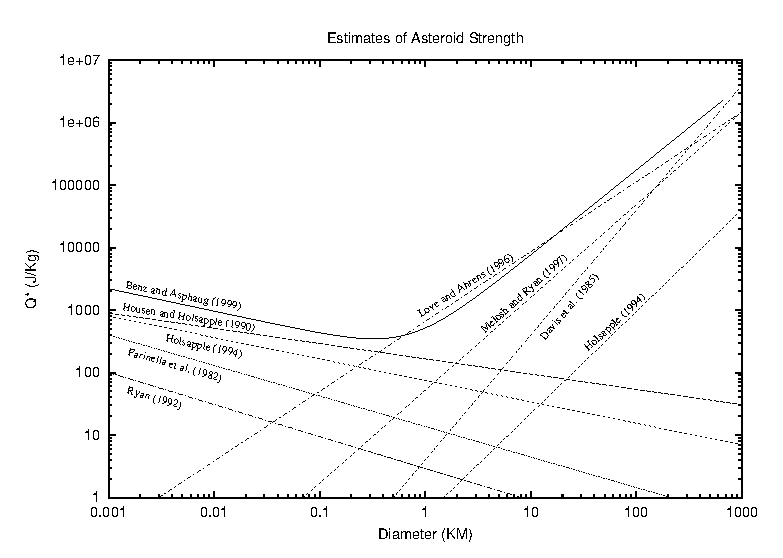
\includegraphics{figure.eps}
%\caption[Short figure caption for LOF]{Sample figure caption (to appear below
%the actual figure). \label{samplefig}}
%\end{center}
%\end{figure}


\chapter{PROGRAMMATIC IMPLEMENTATION\label{prog}}

\section{Program Structure}

The algorithm of obtaining high accuracy wave functions
in the ECG basis set using analytic energy gradient
uses variational principle (\ref{var_principle})
and minimizes functional \ref{functional}.
The structure of the program is shown in Figure \ref{codeflow}.
The presented example has the specifications of non-BO calculation,
but it should be mentioned that the same program structure can be 
utilized for BO calculations with minor input modifications
(exclude masses, include molecular geometry). 

After the program initialization the system specifications
are read in. At this step particle masses need to be 
converted into the pseudoparticle reduced mass matrix,
charges should be stored properly, and a set of 
permutation operators must be constructed from the
symmetry operator.

Since the code is expected to be restarted multiple times
due to computer availability constraints and possible
failures, the current trial wave function expansion
is also stored in the input file. After the system
initialization the basis set can be read in, and 
Hamiltonian and overlap matrices should be computed.
In the next step, secular equation \ref{secular_equation}
needs to be solved to obtain linear expansion coefficients.

After the program processes all the provided data, 
so-called basis building and optimization program (BBOP)
starts. Despite the name, it can contain directives to
calculate single point expectation values and/or perform
various types of the basis set analyses.

\begin{figure}[H]
\begin{center}
\includegraphics[width=140mm]{../pics/CodeFlow.png}
\caption[Code Flowchart]{Code Flowchart. \label{codeflow}}
\end{center}
\end{figure}

The core of the algorithm is an optimization routine.
The user is free to chose different optimization regimes,
which have their advantages and disadvantages. The most
popular choice is to optimize one basis function at a time
and perform several optimization cycles on a given basis
set. In general, any subset of parameters may be chosen for 
optimization. The optimization is driven by 
Newton-Raphson optimization routine, which makes multiple
calls to matrix elements and gradients calculation 
functions.

After the existing basis set is sufficiently optimized, 
new basis functions can be added. One of the possible 
ways to generate it is to perturb the most contributing
function of the existing basis set. After the consecutive
optimization, this function can be added to the basis set.

\section{Performance Considerations}

An immediate observation one can make is that matrix elements
and gradients calculations performed multiple times and are
independent. For that reason a workload can be split between 
the multiple processors and calculations can be performed 
in parallel. 

In sight of the constantly changing computer architecture 
solutions a choice was made in favor of the code portability.
In a simple yet efficient approach communication between
processes is handled by means of Message Passing Interface (MPI).
The up-to-date basis set is maintained and
a copy of the calculated matrix is created on each processor.
After all the processes finish, the individual matrices are merged
on the master process.

It has to be noted that since shared memory solutions become 
available, the number of MPI processes can be reduced in favor 
of OpenMP threads. Such approach, while unlikely to result 
in calculation speed increase, would allow to limit memory 
usage and should be considered for the calculations where
basis set size approaches 15,000 functions.

Another aspect which would allow to increase the speed of individual
matrix element / gradient calculation would be to specify the system
parameters at the compile time. Providing compiler with the information
about exact matrix dimensions would allow to avoid dynamic memory
allocation, speed up functions invocation and improve in-function
caching. A way to do that is to start the code execution by 
running a Python script which reads an input file, updates 
settings file with the system of interest specifications,
recompiles the code and submits the job.






\chapter{FUTURE DIRECTIONS\label{future}}

\section{Muonic Systems}

A great advantage of this procedure developed in appendix \ref{apndx14} 
is that it is applicable to systems with more than three particles. 
For muon-catalyzed fusion, 
for example, the system of real interest is an electron attached 
to the three-body muonic systems treated in that work, 
or certain six-particle systems involving these four-body systems.

Such calculations should be expected in the nearest future.

\section{$\overline{p}dt$}

Another interesting example to consider is a system where
the negative particle has a mass of the same order as the
nuclei (e.g., $\overline{p}dt$). In Table \ref{pdtenergies}
we demonstrate the results obtained for $N$=0 and $N$=1 
states with no vibrational excitation. This system is known
to have only one weekly bound (ground) state 
(\cite{pdt_N1_1}, \cite{pdt_N1_2}) and can be modeled as a
$\overline{p}t$ complex polarized by a deuteron \cite{frolov_pdt}.

In our study we considered this system as a Coulomb
three-body system with unit charges and ignored the 
strong interactions within the system (which are clearly
very important for the extraction of the accurate physical data).
Nevertheless, such calculation is still a viable tool
to estimate to what extent adiabatic and non-adiabatic effects
are taken into account and also make conclusions on 
whether we can expect states to be bound.
 
For $N$=0 level we can compare our results to those obtained
by \cite{frolov_pdt} with the use of a model potential.
It can be seen that the value obtained using explicitly 
correlated Gaussians is lower by \NpdtD  protonic atomic
units. That should probably be attributed to a better 
description of the coupling between the particles 
in the present method than that provided by polarization
potential in \cite{frolov_pdt}. As for the $N$=1 state,
it can be compared to the dissociation energy of the
$\overline{p}dt$ ion, which is easily deduced directly
from the particles' masses. Our calculation suggests that this
system is unbound by \N1pdtD protonic a.u., which
is smaller than the current calculation inaccuracy.
Unfortunately, insufficient numerical precision 
does not allow to take the calculation further and show
the state boundness. 

In future calculations it would be interesting to describe 
strong interactions between the particles and perform the
computation with quadruple precision. 

\begin{table}[t]
\caption[$N$=0 and $N$=1 energies of the $\overline{p}dt$]
{$N$=0 and $N$=1 energies of the $\overline{p}dt$ expressed in
protonic atomic units. $N$=0 energy is compared to the value obtained by
\cite{frolov_pdt}, $N$=1 energy is shown to converge to a value
just above the dissociation energy of $\overline{p}dt$.  }
\centering
\begin{tabular}{r c   r c}
\hline\hline
$N$=0	~~&~~		~~&~~	$N$=1	~~&~~		~~\\
\# of ECGs	~~&~~	Energy	~~&~~	\# of ECGs	~~&~~	Energy	~~\\
\hline
500	~~&~~	-0.381\,190\,892\,903 &~~	250	~~&~~	-0.374\,803\,308\,724 \\
1000	~~&~~	-0.381\,190\,901\,332 &~~	500	~~&~~	-0.374\,803\,346\,392 \\
1500	~~&~~	-0.381\,190\,901\,991 &~~	750	~~&~~	-0.374\,803\,348\,201 \\
2000	~~&~~	-0.381\,190\,902\,159 &~~	1000	~~&~~	-0.374\,803\,348\,292 \\
\hline
\cite{frolov_pdt}~~&~~-0.381190899644 &~~Diss~~&~~-0.374803348316 \\
\hline
\end{tabular}
\label{pdtenergies}
\end{table}

\section{Trinuclear systems}

The diatomic basis functions \ref{N0function} can be easily extended 
to triatomic systems. Such an extension can be achieved by including 
in the Gaussian premultiplier powers of all internuclear distances. 
With that the basis functions are
\begin{equation}
\phi_k = r_1^{2m_k} r_2^{2n_k} r_{12}^{2p_k} \exp [r'(A_k \otimes I_3) r],
\label{3_1}
\end{equation}
where $r_1$ is the distance between the reference nucleus and
nucleus 2, $r_2$ is the distance between the reference nucleus and nucleus 3, 
and $r_{12}$ is the distance between nuclei 2 and 3. 
These functions should be good basis functions for expanding wave functions 
of rotationless (i.e., pure vibrational) states of triatomic systems with 
$\sigma$ electrons, for example, H$_3^+$ , H$_3$, or LiH$_2$. 
They should be able to effectively describe the three types of correlations, 
i.e., the electron-electron, nucleus-nucleus, and nucleus-electron correlations 
in the non-BO calculation.

However, the test calculations showed that the algorithms are not numerically 
stable because they involve oscillating series with finite number of elements 
whose values are large but have opposite signs. We have not been able to overcome 
this problem yet and thus this line of the development is presently on hold. 
In mean time, we have been searching for other alternative types of basis functions 
for use in triatomic non-BO calculations.

One type of functions which can potentially be effective in expanding non-BO 
triatomic wave functions are all-particle Gaussians multiplied by $sin$ and $cos$ 
functions dependent on squares of the internuclear distances:
\begin{equation}
\phi_k = f_1(a_1^k r_1^2 ) f_2(a_2^k r_2^2 ) f_{12}(a_{12}^k r_{12}^2 ) 
\exp [r'(A_k \otimes I_3) r],
\label{3_2}
\end{equation}
where $f_1(a_1^k r_1^2 )$ is either $sin(a_1^k r_1^2 )$ or $cos(a_1^k r_1^2 )$ 
and $f_2$ and $f_{12}$ having analogical forms.

That type of functions was tested in the calculations of bound pure vibrational 
states of a diatomic system with the interaction of the nuclei represented by a 
Morse potential. The test shows that, even though it takes more sin/cos-Gaussians 
than $r^m$-Gaussians to achieve similar precision of the energy, the former functions 
can effectively describe the vibrational states. Future work will involve implementation 
and testing of the sin/cos-Gaussians in all-particle non-BO calculations of the pure
vibrational states of diatomic systems. 
Subsequently, some small triatomics (e.g., H$_3^+$) will also be studied.

% Include the various appendices
\appendix
\chapter{Analytical energy gradient used in variational Born-Oppenheimer calculations with all-electron explicitly correlated Gaussian functions for molecules containing one $\pi$ electron\label{apndx1}}

\includepdf[pages=-]{"../papers/BOpi"}


\chapter{Einstein coefficients for rovibrational transitions of the LiH molecule in the ground X$^1 \Sigma^+$ electronic state\label{apndx2}}

\includepdf[pages={1-},scale=0.8, pagecommand={}]{"../papers/Einstein_coefficients"}


\chapter{An algorithm for quantum mechanical finite-nuclear-mass variational calculations of atoms with L = 3 using all-electron explicitly correlated Gaussian basis functions\label{apndx3}}

\includepdf[pages={1-},scale=0.8, pagecommand={}]{"../papers/L3"}


\chapter{An algorithm for non-Born-Oppenheimer quantum mechanical variational calculations of N = 1 rotationally excited states of diatomic molecules using all-particle explicitly correlated Gaussian functions\label{apndx4}}

\includepdf[pages=-]{"../papers/N1"}


\chapter{Charge asymmetry in rovibrationally excited HD+ determined
using explicitly correlated all-particle Gaussian functions\label{apndx5}}

\includepdf[pages=-]{"../papers/HD+charge_asym"}


\chapter{Lifetimes of rovibrational levels of HD$^+$\label{apndx6}}

\includepdf[pages={1-},scale=0.8, pagecommand={}]{"../papers/Lifetimes"}


\chapter{Charge asymmetry in the rovibrationally excited HD molecule\label{apndx7}}

\includepdf[pages={1-},scale=0.8, pagecommand={}]{"../papers/HD_charge_asym"}


\chapter{Charge asymmetry and rovibrational excitations of HD$^+$\label{apndx8}}

\includepdf[pages={1-},scale=0.8, pagecommand={}]{"../papers/N2"}


\chapter{Nuclear-nuclear correlation function from non-Born-Oppenheimer calculations of diatomic rovibrational states with total angular momentum equal to two (N=2). Charge asymmetry in HD.\label{apndx9}}

\includepdf[pages=-]{"../papers/N2_Correlation_function"}


\chapter{Para-ortho isomerization of H$_2^+$. Non-Born–Oppenheimer direct variational calculations with explicitly correlated all-particle Gaussian functions\label{apndx10}}

\includepdf[pages={1-},scale=0.8, pagecommand={}]{"../papers/H2+"}


\chapter{Non-Born-Oppenheimer method for direct variational calculations of diatomic first excited
rotational states using explicitly correlated all-particle Gaussian functions\label{apndx11}}

\includepdf[pages=-]{"../papers/H2"}


\chapter{Direct non-Born-Oppenheimer variational calculations of all bound vibrational states corresponding to the first rotational excitation of D$_2$ performed with explicitly correlated all-particle Gaussian functions\label{apndx12}}

\includepdf[pages={1-},scale=0.8, pagecommand={}]{"../papers/D2"}


\chapter{Ortho–para nuclear-spin isomerization energies for all bound vibrational states of ditritium (T$_2$) from non-Born–Oppenheimer variational calculations performed with explicitly correlated all-particle Gaussian functions\label{apndx13}}

\includepdf[pages=-]{"../papers/T2"}


\chapter{Non-Born–Oppenheimer variational method for calculation of rotationally excited binuclear systems\label{apndx14}}

\includepdf[pages=-]{"../papers/x_i"}


\chapter{A comparison of two types of explicitly correlated Gaussian functions for
non-Born-Oppenheimer molecular calculations using a model potential\label{apndx15}}

\includepdf[pages=-]{"../papers/sin_basis"}




% Switch the spacing to single-spaced for the references
\renewcommand{\baselinestretch}{1}		% chaning the value
\small\normalsize						% switch size to make the value take

% this is how pdf documents can be included
%\includepdf[pages=-]{"../papers/H2"}
%\includepdf[pages=-]{"../papers/D2"}

% Create the References list
\bibliographystyle{uabibnat}
\bibliography{bibliography}

\end{document}
